%----------------------------------------------------------------------------------------
%  Validation of AI-generated results in theoretical physics
%  ICML 2026 AI and Physics Workshop  --  Michael R. Douglas
%  Reuses the CleanEasy beamer theme from ../qft-formalization-talk
%----------------------------------------------------------------------------------------
\documentclass[aspectratio=169,xcolor=dvipsnames]{beamer}
\makeatletter
\def\input@path{{theme/}{configs/}{./}}
\makeatother
\graphicspath{{./}}
\usetheme{CleanEasy}
\usepackage[utf8]{inputenc}
\usepackage{lmodern}
\usepackage[T1]{fontenc}
\usepackage{fix-cm}
\usepackage{amsmath}
\usepackage{mathtools}
\usepackage{listings}
\definecolor{keywordcolor}{rgb}{0.5, 0.1, 0.1}
\definecolor{tacticcolor}{rgb}{0.1, 0.2, 0.4}
\definecolor{commentcolor}{rgb}{0.4, 0.4, 0.4}
\definecolor{symbolcolor}{rgb}{0.0, 0.1, 0.6}
\definecolor{sortcolor}{rgb}{0.1, 0.5, 0.1}
\definecolor{attributecolor}{rgb}{0.7, 0.1, 0.1}
\def\lstlanguagefiles{lstlean.tex}
\usepackage{xcolor}
\usepackage{hyperref}
\usepackage{graphicx}
\usepackage{booktabs}
\usepackage{tikz}
\usetikzlibrary{positioning, shapes, arrows, calc, decorations.pathreplacing, arrows.meta, backgrounds}
\usepackage{etoolbox}
%
\def\blue{\color{blue}}
\def\p{\\[0.1in] \pause}
\newcommand{\be}{\begin{equation*}}
\newcommand{\ee}{\end{equation*}}
\def\BR{\mathbb{R}}
\def\E{{\mathbb E}}
%
\input{configs}
%----------------------------------------------------------------------------------------
\title[Validating AI in physics]{Validation of AI-generated results\\ in theoretical physics}
\subtitle{ICML 2026 -- AI and Physics Workshop}
\author[MRD]{Michael R. Douglas}
\institute[CMSA]{CMSA, Harvard University \;\&\; AletheAI}
\date{}
\titlegraphic{%
  \begin{tikzpicture}[remember picture, overlay]
    \node[anchor=north east, xshift=-0.8cm, yshift=-0.3cm] at (current page.north east)
      {
\includegraphics[height=1.0cm]{cmsa-logo.png}};
  \end{tikzpicture}}
%----------------------------------------------------------------------------------------
\begin{document}

\begin{frame}[plain]
  \titlepage
  \begin{tikzpicture}[remember picture, overlay]
    \node[anchor=north] at ([yshift=-0.95in]current page.center) {%
      \begin{minipage}{0.82\paperwidth}
        \centering\scriptsize\itshape
        AI now generates physics results faster than we can check them.  A central part of
        the answer: machine-checkable \emph{certificates}, not human reading alone.  A survey
        of AI for mathematics and physics, and of formalization as the validation technology.
      \end{minipage}};
  \end{tikzpicture}
\end{frame}

\begin{frame}[plain]{Contents}
  \tableofcontents
\end{frame}

%======================================================================
\section{The validation problem}
%======================================================================
\begin{frame}{A scenario}
We are LHC physicists.  We want the scattering amplitude for
$2\text{ partons}\to 6\text{ gluons}+W$, to interpret our data. \p

We ask GPT-10.  It writes a 1000-page program and computes the result numerically
in a day. \p

Do we trust it?  At present, no -- and for good reason. \p

Understanding the program well enough to rely on it will take us {\bf far longer}
than it took the AI to write it.  Our ability to {\bf validate} has become the bottleneck.
\end{frame}

\begin{frame}{The thesis}
AI is changing the \emph{economics} of research: generation is becoming cheap,
validation is not. \p

\begin{itemize}
  \item Statistical models make some errors unavoidable; research itself generates
        ideas that must be tested, and some are wrong.
  \item Humans have protocols for this -- but they do not transfer to AI, and the
        goal is still to convince \emph{humans} of correctness.
\end{itemize}\pause\medskip

\begin{block}{Claim}
An \textbf{algorithm-checkable certificate} -- a deterministic, near-$100\%$-reliable check,
cheaper than the derivation (\emph{not} an LLM checking an LLM) -- must become a
\emph{central component} of trust: the part that scales when we can no longer read the
output by hand.
\end{block} \pause

\smallskip
What is new is not the idea of checking -- it is that AI makes \emph{generation} so cheap
that \textbf{checking, not generating, becomes the bottleneck.}
\end{frame}

%======================================================================
\section{Recent progress: AI for mathematics and physics}
%======================================================================
\begin{frame}{The state of AI, 2025--2026}
\begin{itemize}
  \item LLMs were optimized for next-word prediction (through GPT-4); performance jumped
        with RL on new reward signals -- reasoning, coding, tool use.
  \item Roughly $100$ Elo points/year on public arenas; early-2026 models
        (Claude Opus 4.5+, Gemini 3 Pro, GPT-5) far stronger than 2024.
  \item Excellent at retrieval and adapting known arguments; weaker at original logical
        reasoning -- much current work uses search, verification and self-check to compensate.
  \item Strongest in high-resource domains (Python); weaker in low-resource ones
        (most academic specialties).
\end{itemize} \pause
\smallskip
The frontier crossed a threshold for research-level math in late 2025.
\end{frame}

\begin{frame}{AI for mathematics -- impressive, but unverified}
\textbf{IMO 2025:} both OpenAI and Google DeepMind reached gold-medal level
(35/42, 5 of 6 problems), with \emph{general-purpose} reasoning models writing
natural-language proofs. \p

A landmark for reasoning.  But: to trust a natural-language proof, {\bf you have to read it.} \p

\pause
Whether AI can \emph{do} mathematics is a deep question in its own right -- but the
question for \emph{this} talk is \textbf{``how do we know the answer is right?''}
\end{frame}

\begin{frame}[fragile]{Background -- interactive theorem provers and Lean}
The ``verified'' results that follow rely on one tool, new to most physicists.
An \textbf{interactive theorem prover (ITP)} is a language for stating definitions and
theorems and \emph{proving} them, where a \textbf{fixed algorithm} checks every step -- so a
checked proof is essentially $100\%$ reliable, and \textbf{interpretable}.  You work at a high
level (via ``tactics''), much as on paper.  A proof looks like:
\smallskip
{\scriptsize
\begin{lstlisting}[language=lean]
theorem infinite_primes (n : ℕ) : ∃ p, n ≤ p ∧ Prime p :=
  let p := minFac (n ! + 1)
  have f1 : n ! + 1 ≠ 1 := ne_of_gt <| succ_lt_succ <| factorial_pos _
  have pp : Prime p := minFac_prime f1
  have np : n ≤ p :=
    le_of_not_ge fun h =>
      have h₁ : p | n ! := dvd_factorial (minFac_pos _) h
      have h₂ : p | 1 := (Nat.dvd_add_iff_right h₁).2 (minFac_dvd _)
      pp.not_dvd_one h₂
  ⟨p, np, pp⟩
\end{lstlisting}}
\end{frame}

\begin{frame}{Lean and mathlib -- what has been formalized}
\textbf{Lean 4} is the leading system for mathematics; its library \textbf{mathlib}
($\sim$2M lines) spans much of the undergraduate curriculum and well beyond.  Landmarks:
\begin{itemize}
  \item Four-Colour and Feit--Thompson theorems (Gonthier \emph{et al}); the Kepler
        conjecture (Hales, Flyspeck).
  \item Scholze--Clausen liquid tensor experiment (Commelin \emph{et al}); polynomial
        Freiman--Ruzsa (Gowers, Green, Manners, Tao); Carleson's theorem (2025).
  \item In progress: Fermat--Wiles (Buzzard).  Physics formalization is just beginning
        (more shortly).
\end{itemize} \pause
\smallskip
A growing community uses Lean -- and, increasingly, AI agents write it, removing the cost
that for two decades made this a specialist's tool. \pause
\smallskip
The point to carry forward: a Lean-checked proof is a \textbf{machine-checkable certificate.}
\end{frame}

\begin{frame}{AI for mathematics -- now verified}
\textbf{AlphaProof Nexus} (DeepMind, arXiv:2605.22763, May 2026): LLM agents $+$ Lean.
\begin{itemize}
  \item Solved \textbf{9 of 353} open Erd\H{o}s problems (one open 56 years),
        \textbf{44 of 492} OEIS conjectures, a 15-year-old algebraic-geometry question.
  \item $\sim$ a few hundred dollars per problem.
  \item Every proof is mechanically checked by Lean -- \emph{no expert review of the logic needed}.
\end{itemize} \pause
\smallskip
The model that matters: \textbf{LLM generates, the proof assistant certifies.} \p

(Humans still vet that the formal \emph{statement} captures the conjecture -- hold that thought.)
\end{frame}

\begin{frame}{Certificate by construction}
\textbf{AlphaEvolve} (DeepMind, 2025) and \textbf{FunSearch}: evolutionary search where a
candidate is kept only if it \emph{passes an exact evaluator}.
\begin{itemize}
  \item $4\times4$ complex matrix multiply in 48 multiplications -- first improvement on
        Strassen in 56 years.
  \item Matched or beat the state of the art on $\sim 20\%$ of $50+$ open problems
        (incl.\ the 11-D kissing number).
\end{itemize} \pause
\smallskip
Here the result is \textbf{trustworthy by construction}: the certificate \emph{is} the check
the search optimizes against.  The purest form of ``trust the output, not the generator.''
\end{frame}

\begin{frame}{Scale -- and a skeptic}
\textbf{Equational Theories Project} (Tao, 2024): $22$M universal-algebra questions,
settled with Lean + automated provers; humans needed only for the stubborn tail. \p

\textbf{The Erd\H{o}s sweep} (2025--26): Erd\H{o}s \#728 resolved autonomously in Lean
(Aristotle); automated literature + proof search closing ``open'' problems weekly. \p
\pause
Tao's caution is worth quoting: automation first harvests the \emph{lowest-hanging fruit};
formalization is what keeps the harvest \emph{honest}.
\end{frame}

\begin{frame}{AI for physics (1) -- generating results}
AI is now producing \emph{physics}, not just mathematics. Two Harvard examples:
\smallskip
\begin{itemize}
  \item \textbf{Scattering amplitudes} (Schwartz, Cheung, Dersy; IAIFI).
        Transformers predict coefficients in the amplitude bootstrap for planar
        $\mathcal{N}=4$ super Yang--Mills (arXiv:2405.06107); symbolic regression
        ``learns the simplicity'' of amplitudes, distilling huge expressions to
        compact closed forms (arXiv:2408.04720).
  \item \textbf{Discovery by program search} (Brenner; Harvard \& Google).
        \textbf{FunSearch} -- an LLM proposing programs, scored by an evaluator --
        found record cap sets and new constructions; related work learns PDE
        discretizations and effective models.
\end{itemize} \pause
\smallskip
\textbf{The validation question, attached to each:} a transformer's amplitude
coefficient $\to$ must satisfy bootstrap / known-limit constraints; a distilled
formula $\to$ a closed form you can \emph{check}; FunSearch $\to$ kept only if the
\emph{exact evaluator} passes.
\end{frame}

\begin{frame}{AI for physics (2) -- and where the certificate is missing}
Many-body and geometry, where the check is numerical:
\begin{itemize}
  \item \textbf{Neural quantum states}: variational ans\"atze for lattice systems --
        the \emph{variational energy upper bound} is a built-in certificate.
  \item \textbf{ML for lattice QCD}: gauge-equivariant nets, flow-based sampling;
        validated by standard Monte-Carlo cross-checks.
  \item \textbf{Symbolic distillation of Calabi--Yau metrics} (arXiv:2602.07834):
        a 5-term formula, $R^2=0.9994$, validated against \emph{physical observables}
        (volumes, Yukawa couplings).
\end{itemize} \pause
\smallskip
The trustworthy results are exactly the ones \textbf{carrying a cheap check}.
The danger case -- a fluent LLM ``derivation'' with \emph{no} certificate -- is
the one physics culture is least equipped to catch.
\end{frame}

\begin{frame}{AI for physics (3) -- the validation showcase}
\textbf{The generalized quantum Stein's lemma, formalized in Lean}
(Meiburg \emph{et al}, arXiv:2510.08672).
\begin{itemize}
  \item A central theorem of quantum information -- the operational meaning of relative
        entropy, and the reversibility of quantum resources.
  \item Its original proof (2010) was found to have a \textbf{gap} (Quantum 2023);
        re-proved by Hayashi--Yamasaki (2024).
  \item Now \textbf{machine-verified} -- the most technically demanding physics theorem
        formalized to date -- and the formalization \emph{itself rectified further
        imprecisions} in the proof.
\end{itemize} \pause
\bigskip
\begin{center}
\large gap $\;\to\;$ reproof $\;\to\;$ machine-checked $\;\to\;$ caught more
\end{center}
\smallskip
This arc is the whole thesis: formalization does not just certify -- it \textbf{finds the errors}.
\end{frame}

\begin{frame}{AI for physics (3, cont.) -- the formalization landscape}
\begin{itemize}
  \item \textbf{PhysLean} (Tooby-Smith \emph{et al}): Wick's theorem, the Higgs potential,
        Maxwell's equations, Lorentz-group index notation.
  \item \textbf{Quantum information} in Lean -- the library built for the Stein result.
  \item \textbf{Our QFT work} -- OSforGFF (4D free QFT, all OS axioms) and a lattice
        Yang--Mills mass gap -- verified mathematical physics; details shortly.
\end{itemize} \pause
\smallskip
Small but real, and growing fast.  Almost all of it formalizes \emph{rigorous} physics --
the hard, unmapped territory is everything else, which is most of physics.
\end{frame}

\begin{frame}{Survey takeaway}
\begin{block}{}
Across math and physics, the AI results we \emph{trust} are exactly the ones that
came with a \textbf{check}.
\end{block} \pause
\begin{itemize}
  \item Lean-certified proofs; exact-evaluator search; variational bounds; agreement with
        known observables.
  \item Where there is no certificate -- a fluent natural-language derivation -- we are back
        to reading, and back to the bottleneck.
\end{itemize} \pause
\smallskip
Physics has the \textbf{least-developed certificate machinery} of any quantitative field.
That is the problem -- and the opportunity.
\end{frame}

%======================================================================
\section{What is validation?}
%======================================================================
\begin{frame}{What ``validation'' means}
Two things at once:
\begin{itemize}
  \item the result is \textbf{correct}, and
  \item we can \textbf{convince} the users/stakeholders that it is.
\end{itemize}\pause\medskip
\pause
The enabling fact is an \textbf{asymmetry}: checking can be far cheaper than finding.
\begin{itemize}
  \item \textbf{SAT}: a satisfying assignment is its own certificate -- trivial to check, hard to find.
  \item \textbf{UNSAT}: the certificate is a proof.
\end{itemize}
This is the content of $P \ne NP$. \pause
\smallskip

Crucially, the check is by a \textbf{fixed algorithm} -- deterministic, essentially $100\%$
reliable, and simple enough that \textbf{we can understand and trust the checker itself} --
\emph{not} by another, fallible, LLM.  You cannot cure an LLM's errors with a second LLM. \pause
\smallskip

Validation technology $=$ systematically attaching \textbf{cheap, algorithm-checkable
certificates} to expensive results.
\end{frame}

%======================================================================
\section{The validation toolbox}
%======================================================================
\begin{frame}{Verified symbolic computation}
\textbf{Beyond formal proof}, a second technology.  Computer algebra (Mathematica, SageMath)
is everywhere in physics -- but it is \textbf{not constrained to sound manipulations.} \p
\pause
Define a quantity two ways:
\begin{center}
\texttt{a = <defn 1> ; b = <defn 2>} \qquad vs.\qquad
\texttt{b = <defn 1> ; a = <defn 2>}
\end{center}
(with later references to \texttt{a}, \texttt{b} unchanged). \\
The CAS \textbf{does not know or care} which is right.  An ITP does -- the types must match. \p
\pause
\textbf{Opportunity:} have the CAS emit a \emph{certificate} of its steps that Lean can check --
keeping CAS speed, gaining ITP soundness.
\end{frame}

\begin{frame}{Verified numerical computation}
Approximate, yet rigorous: round \emph{outward} and propagate.
\begin{itemize}
  \item Interval arithmetic: replace $x$ by rigorous bounds $[a,b]$, propagate through every op.
  \item \textbf{Lorenz attractor} is chaotic (Tucker 2002; verified in Isabelle/HOL by Immler 2018).
  \item \textbf{Verified Calabi--Yau metric}: neural net finds an approximate solution; rigorous
        spectral-gap and error bounds + a fixed-point theorem $\Rightarrow$ an exact solution exists.
\end{itemize}
\begin{center}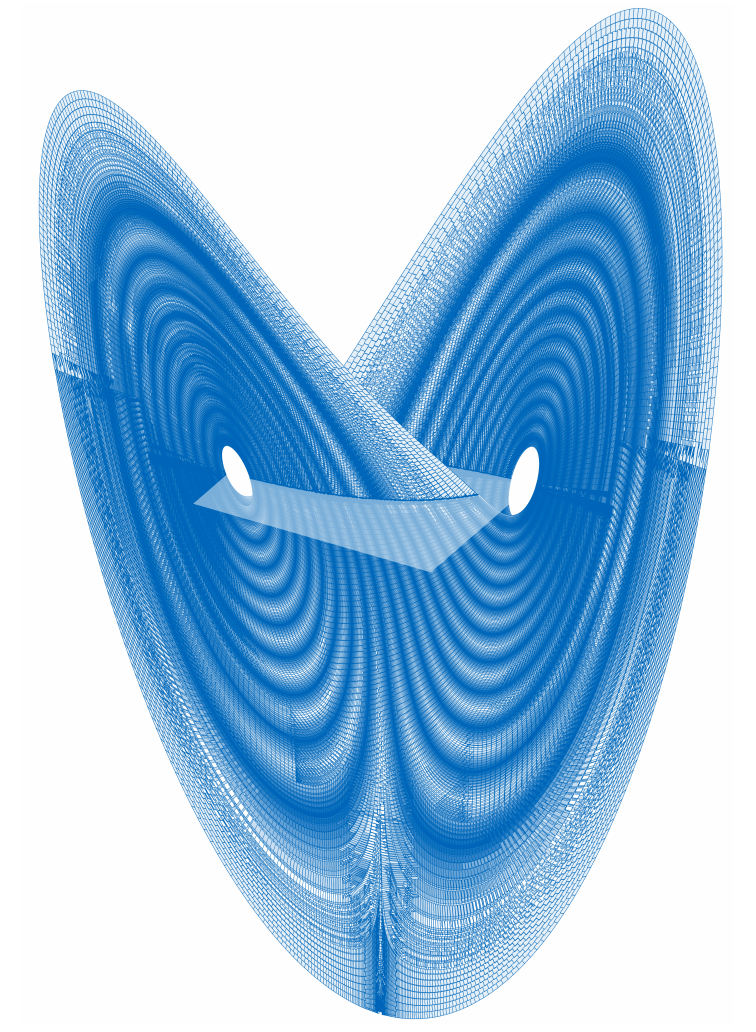
\includegraphics[height=1.25in]{lorenz.png}\end{center}
\pause
\vskip -0.15in
\emph{Honest caveat:} verified numerics inside ITP is still thin.
Near-term: couple validated computation to an ITP so there is at least a \textbf{specification}.
\end{frame}

%======================================================================
\section{Is physics ready?}
%======================================================================
\begin{frame}{Act 1 -- what can be formalized at all?}
A natural criterion for \emph{scope}, not for trust: a result can be formalized iff it has a
\textbf{mathematically well-defined formulation} -- \emph{not} a rigorous justification.
\begin{itemize}
  \item Setting a Lagrangian term to zero: not rigorous, but well-defined -- formalizable.
  \item The path integral's \emph{steps} are well-defined, even where the object is not.
  \item ``Approximate 1200 by 1000 but not by 800'': hard to even formulate.
\end{itemize} \pause
\smallskip
This says what is \emph{in range} -- not what is \emph{correct}.  Well-definedness is
\textbf{necessary but nowhere near sufficient for trust}: one can formalize the steps of a
path-integral calculation and certify \emph{nothing} about the physics.  Closing that gap
is the rest of this section.
\end{frame}

\begin{frame}{Act 2 -- rigorous, or merely well-defined?}
Two regimes need different paradigms:
\begin{itemize}
  \item \textbf{Verified mathematical physics} -- rigorous results; the mathematician's
        paradigm applies directly (stability of matter, CPT, our OS construction).
  \item \textbf{Verified physical computation} -- collider amplitudes, bootstrap bounds,
        dynamical-systems bounds; needs verified CAS + numerics + a specification.
\end{itemize} \pause
\smallskip
\textbf{Key point:} you do \emph{not} have to solve the foundations to validate a calculation.
Costello (and others) showed perturbative QFT \emph{can} be made rigorous order-by-order --
a possibility result, not a prescription -- even though \emph{constructing} the full theory
is a Millennium Problem. \p
$\Rightarrow$ the Standard-Model amplitudes experimentalists actually use are a realistic target.
\smallskip\pause
But a rigorous \emph{derivation} is still not a trusted \emph{result} -- that turns on the
specification.
\end{frame}

\begin{frame}{Act 3 -- formalizable $\ne$ validated (the gap)}
A formal proof certifies an \emph{implication}:
\be
A, B, C \;\Longrightarrow\; X, Y, Z.
\ee
It does \textbf{not} certify that $A,B,C$ and $X,Y,Z$ mean what we intend. \p
\pause
\begin{itemize}
  \item From contradictory assumptions one can prove anything -- the checker is happy.
  \item Formalizing the \emph{steps} of a path-integral calculation verifies a record of the
        steps, not the physical result.
\end{itemize} \pause
\smallskip
\begin{block}{The specification / meaning gap}
The real work -- and the real research frontier -- is writing formal specifications that
\textbf{human experts vet} as capturing the physics.  This is what everyone else skips.
\end{block}
\end{frame}

\begin{frame}{So what does formalization actually buy you?}
The skeptic's objection: haven't we just moved the trust from the proof to the spec? \p
\pause
Yes -- and that \emph{is} the point.  Formalization does not eliminate trust; it
\textbf{relocates and shrinks} it.
\begin{itemize}
  \item \textbf{Before:} trust a 1000-page AI derivation you cannot read.
  \item \textbf{After:} trust a \emph{short, explicit specification} $+$ a tiny proof kernel.
        Everything in between is machine-checked.
\end{itemize} \pause
\smallskip
The specification is small, stable, reusable, and \textbf{independently auditable} -- including
against physics' own battery: symmetries, limiting cases, dualities, numerics. \pause
\begin{block}{}
Trust $=$ a formal certificate of the derivation $+$ a specification that survives the
physicist's consistency checks.  Not certainty -- a drastic, auditable reduction of what
you must take on faith.
\end{block}
\end{frame}

\begin{frame}{Worked example -- the collider amplitude, made precise}
Back to the opening: the amplitude for $g\,g \to W + 6\,g$ at the LHC. \p
\pause
What would a \textbf{specification} -- the textbook definition we already trust -- say?
\begin{itemize}
  \item $\mathcal{M}$ is the order-$\alpha_s^{k}$ term of the Standard-Model perturbative
        expansion for this external state -- which \emph{can} be made rigorous order-by-order
        (cf.\ Costello; we need not adopt his framework).
  \item It must satisfy the physics that pins it down:
  \begin{itemize}
    \item \textbf{Gauge invariance}: replace a gluon polarization $\epsilon_i \to p_i$ and
          the amplitude must vanish (Ward identity).
    \item \textbf{Bose symmetry} under exchange of identical gluons.
    \item Correct \textbf{soft / collinear} (infrared) singularities and factorization.
  \end{itemize}
\end{itemize} \pause
\smallskip
These consistency conditions are not decorations -- they are most of the specification.
\end{frame}

\begin{frame}{Worked example -- validating the 1000-page program}
The AI writes the program; the machine checks it against the spec.
\begin{itemize}
  \item \textbf{Verified symbolic computation}: the colour / Lorentz / Dirac algebra and the
        Feynman-rule bookkeeping emit Lean-checkable certificates.
  \item \textbf{Verified numerics}: the loop / phase-space integration with rigorous
        (interval) error bounds, or post-verified.
  \item \textbf{Physics consistency checks}, run automatically: Ward identity $=0$;
        agreement with known lower-multiplicity and soft limits; gauge-parameter independence.
\end{itemize} \pause
\smallskip
\textbf{Trusted surface:} a short textbook specification $+$ the proof kernel.  The
1000-page program is machine-checked against it -- and nobody has to read it. \pause
\smallskip
\begin{center}\emph{The bottleneck from the opening -- dissolved.}\end{center}
\end{frame}

\begin{frame}{The deep frontier -- foundations for physical reasoning}
Physicists rarely write rigorous proofs, yet the community reaches \textbf{stable agreement}
on what is established.  Perhaps physical reasoning, at its best, is already rigorous --
just not grounded in ZFC. \p
\pause
A program: make those foundations explicit and formal.
\begin{itemize}
  \item Formalize axiomatic QM/QFT; verify that a claimed observation conflicts with them
        (e.g.\ a CPT violation -- which axiom must give?).
  \item Admit well-supported but unproven statements as \textbf{axioms} -- asymptoticity of
        perturbation series, $S$-duality, AdS/CFT -- and let the verifier \textbf{detect contradiction}.
\end{itemize} \pause
\smallskip
Explicit axioms do not make the conjectures \emph{true} -- they make the \textbf{dependency
structure} checkable: which results rest on which conjectures, and where a surprise would
propagate.  This is where validation of AI-generated physics becomes genuinely new.
\end{frame}

\begin{frame}{Example -- codifying the lore behind an exact result}
Formalizing \emph{rigorous} physics (our free-QFT and lattice Yang--Mills results) is the
mature end.  The deeper frontier is the \emph{non-rigorous} reasoning physicists trust anyway. \pause
\medskip

\textbf{Seiberg--Witten} (1994): the \emph{exact} low-energy solution of $\mathcal{N}=2$
$SU(2)$ super Yang--Mills.  The derivation is not rigorous; its physical ``axioms'':
\begin{itemize}
  \item holomorphy of the prepotential (from $\mathcal{N}=2$ supersymmetry);
  \item the Coulomb branch has \emph{exactly} the expected singularities -- massless
        monopoles / dyons;
  \item electric--magnetic duality: the monodromies must compose consistently;
  \item matching onto weak-coupling (one-loop $+$ instanton) asymptotics.
\end{itemize} \pause
\smallskip
Why it is trusted: \textbf{independent agreement} across perturbation theory, semiclassics /
instantons (Nekrasov's instanton sum reproduces the prepotential), and the exact answer.
\smallskip

Codify those axioms $\Rightarrow$ the reasoning becomes \textbf{auditable}; a verifier checks
the chain and flags contradiction.  The pert.\,/\,instanton\,/\,exact triangle, made formal.
\end{frame}

%======================================================================
\section{It is real}
%======================================================================
\begin{frame}{Evidence (1) -- a verified construction of QFT}
\textbf{OSforGFF} (with Hoback, Mei, Nissim): formalize the $4$D massive free Euclidean
QFT and verify the Osterwalder--Schrader axioms.
\begin{itemize}
  \item Construct an infinite-dimensional Gaussian measure with covariance
        $C(x,y)=\int \! d^4k\, e^{ik(x-y)}/(k^2+m^2)$.
  \item \textbf{All five OS axioms + ergodicity. 0 sorries, 0 axioms.} $\sim$32{,}000 lines.
  \item Minlos' theorem and Schwartz nuclearity proved from scratch along the way.
\end{itemize} \pause
\smallskip
A physics result, certified to the same standard as formalized mathematics.
\end{frame}

\begin{frame}{Evidence (2) -- a Yang--Mills mass gap, and the pace of change}
\textbf{lgt} (with Rajasekaran): $U(n)$ Wilson lattice Yang--Mills, exponential
correlation decay at strong coupling via Dobrushin uniqueness.
\begin{itemize}
  \item Mass-gap theorems fully proved, \textbf{0 project axioms}.
  \item Eight sorry-free layers: lattice geometry $\to$ Gibbs/DLR $\to$ Dobrushin decay $\to$ mass gap.
\end{itemize} \pause
\smallskip
And the trajectory: \textbf{Bochner's theorem} was proved by Claude Code in $\sim$2 days,
\emph{nearly autonomously}, in February 2026.  A year earlier this was unthinkable.
\end{frame}

%======================================================================
\section{Challenges and outlook}
%======================================================================
\begin{frame}{The hard parts}
\begin{itemize}
  \item \textbf{The specification gap} again: who writes, and who vets, the formal statement of
        ``the physical scattering amplitude''?
  \item \textbf{Who validates the validator?}  An \emph{LLM} judge can be reward-hacked
        (Goodhart); a deterministic proof \emph{kernel} cannot -- it is small, fixed, and
        auditable.  The residual risk collapses onto the \textbf{specification}.
  \item \textbf{The insidious failure:} models led astray by nearly-but-not-quite-right analogies
        -- complex-matrix results applied over a Grassmann algebra; conditionally convergent
        treated as absolutely convergent.
\end{itemize} \pause
\smallskip
\textbf{Countermeasures that work today:} cross-model validation; unit tests for new definitions;
back-chaining through vetted ``textbook axioms.''
\end{frame}

\begin{frame}{Outlook}
\begin{itemize}
  \item The bottleneck in knowledge formation is shifting from discovery and writing to
        \textbf{selecting, reading and validating}.
  \item For physics: build the certificate machinery -- verified CAS, verified numerics,
        formalized specifications, libraries of formalized physics.
  \item For the ML community: \textbf{autoformalization}, \textbf{certificate-emitting CAS}, and
        \textbf{verified numerics in ITP} are rich, underworked, open problems.
\end{itemize} \pause
\bigskip
\begin{center}
\emph{The question is no longer ``can it be done,'' but ``what should we validate next?''}
\end{center}
\end{frame}

\begin{frame}{Conclusions}
\begin{itemize}
  \item AI generates physics faster than we can check it; \textbf{machine-checkable
        certificates} must become a central component of trust -- alongside expert-vetted
        specifications and physics' own consistency checks.
  \item Formalization -- formal proof, verified symbolic, verified numerical computation --
        is the validation technology, and it is \textbf{working now} at research level.
  \item Physics is more ready than it looks: you need not solve the foundations to validate
        a calculation.
  \item The frontier is \textbf{meaning}: formalizable is not validated.  Specifications,
        vetted by experts, are the real work -- and where ``foundations for physical reasoning''
        could make this genuinely new.
\end{itemize}
\end{frame}

\end{document}
